\chapter{IoT Gateway}\label{chap:iotgateway}

Das IoT Gateway dient dazu einzelne Messpunkte zusammen zufassen und die Daten danach ins Internet zu übertragen. Als Gateway Hardware nutzen wir die bekannte Embedded Platform Beagle Bone Black. Dies ermöglicht uns auch vorhandene Erweiterungen zu nutzen. Das Gateway arbeitet mit zwei verschiedenen Methoden um die einzelnen Messpunkte abfragen zu können. Einerseits dem CAN-Bus, welcher in der Automobiltechnik sehr verbreitet ist und anderseits eine Bluetooth Smart Schnittstelle um die Sming Messknoten ansprechen zu können. Die Übertragung ins Internet wird mithilfe eines UMTS-Routers gemacht.


%Unser Internet of Things Gateway besteht wiederum aus mehreren Teilen. Die einzelnen Sensoren werden entweder über den CAN-Bus oder an ein Sming angeschlossen. Der CAN-Bus wird von uns über ein BeagleBone Cape mitgelesen. Die Daten des Smings können wir ebenfalls auf dem BeagleBone empfangen. Dies erreichen wir mit Hilfe des Bluetooth Smart USB Dongle BLED112 von Bluegiga, welcher am BeagleBone angeschlossen wird.

\begin{figure}[hbtp]
    \center
    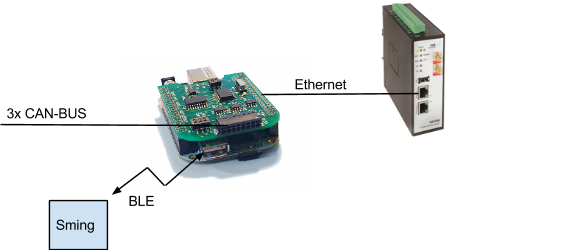
\includegraphics[width=\textwidth]{bilder/aufbau_in_auto.png}
    \caption{Aufbau des IoT Gateways}
    \label{fig:aufbau_iot_gateway}
\end{figure}

\section{Netmodule NetBox NB1600}\label{sec:netbox}
Als UMTS-Router setzen wir auf den Netmodule Router NB1600. Dieser kam schon in unserem Schwerpunkt Mobile Computing beim Semesterprojekt "Smoje" zum Einsatz. Für unseren Einsatzzweck als reine Bridge zwischen Ethernet und UMTS-Netz wird er nicht ausgelastet. Der NB1600 könnte nähmlich auch noch GPS empfangen und als Wlan-Hotspot dienen. Daher besteht hier noch eine Optimierungsmöglichkeit durch den Einsatz eines geigneten USB Dongles der direkt vom Beagle Bone aus auf UMTS zugreifen kann. Dieser zu evaluieren hätte aber den Zeitrahmen für das Projekt gesprengt.

\begin{figure}[hbtp]
	\center
	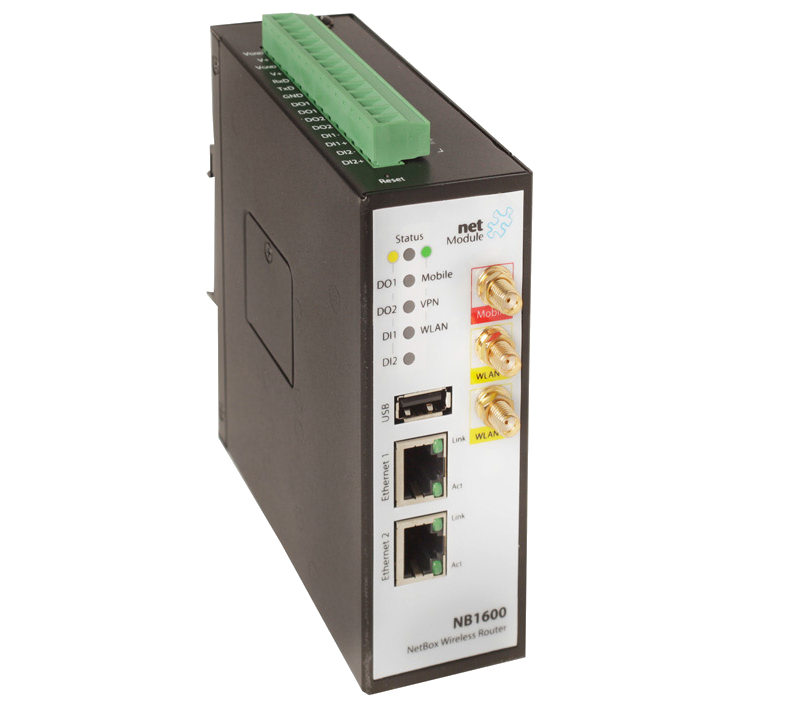
\includegraphics[width=6cm]{bilder/netmodule.png}
	\caption{Foto NetModule NB1600}
	\label{fig:netbox}
\end{figure}


\section{CAN-Cape}
%Als Basis für unsere Software kommt ein BeagleBone Black als Recheneinheit zum Einsatz. Zum Anschliessen der drei CAN-Busse des Fahrzeuges verwenden wir ein von einem Italiener gefertigtes CAN-Cape, dass einfach auf das Beaglebone drauf gesteckt werden kann:

 Der CAN-Bus wird im Bern Formula Student Projekt genutzt um die Steuerbefehle innerhalb des Autos zu übertragen. Es werden drei seperate Verdrathungen geführt. Wir empfangen die Daten der 3 CAN-Busse über das Beagle Bone Black CAN Cape von Tower Tech. Da die ganze Steuerung des Autos über die CAN-Busse läuft haben wir nur lesenden Zugriff. Die Installationsanleitung zum Cape befindet sich im Anhang.

\begin{figure}[hbtp]
	\center
	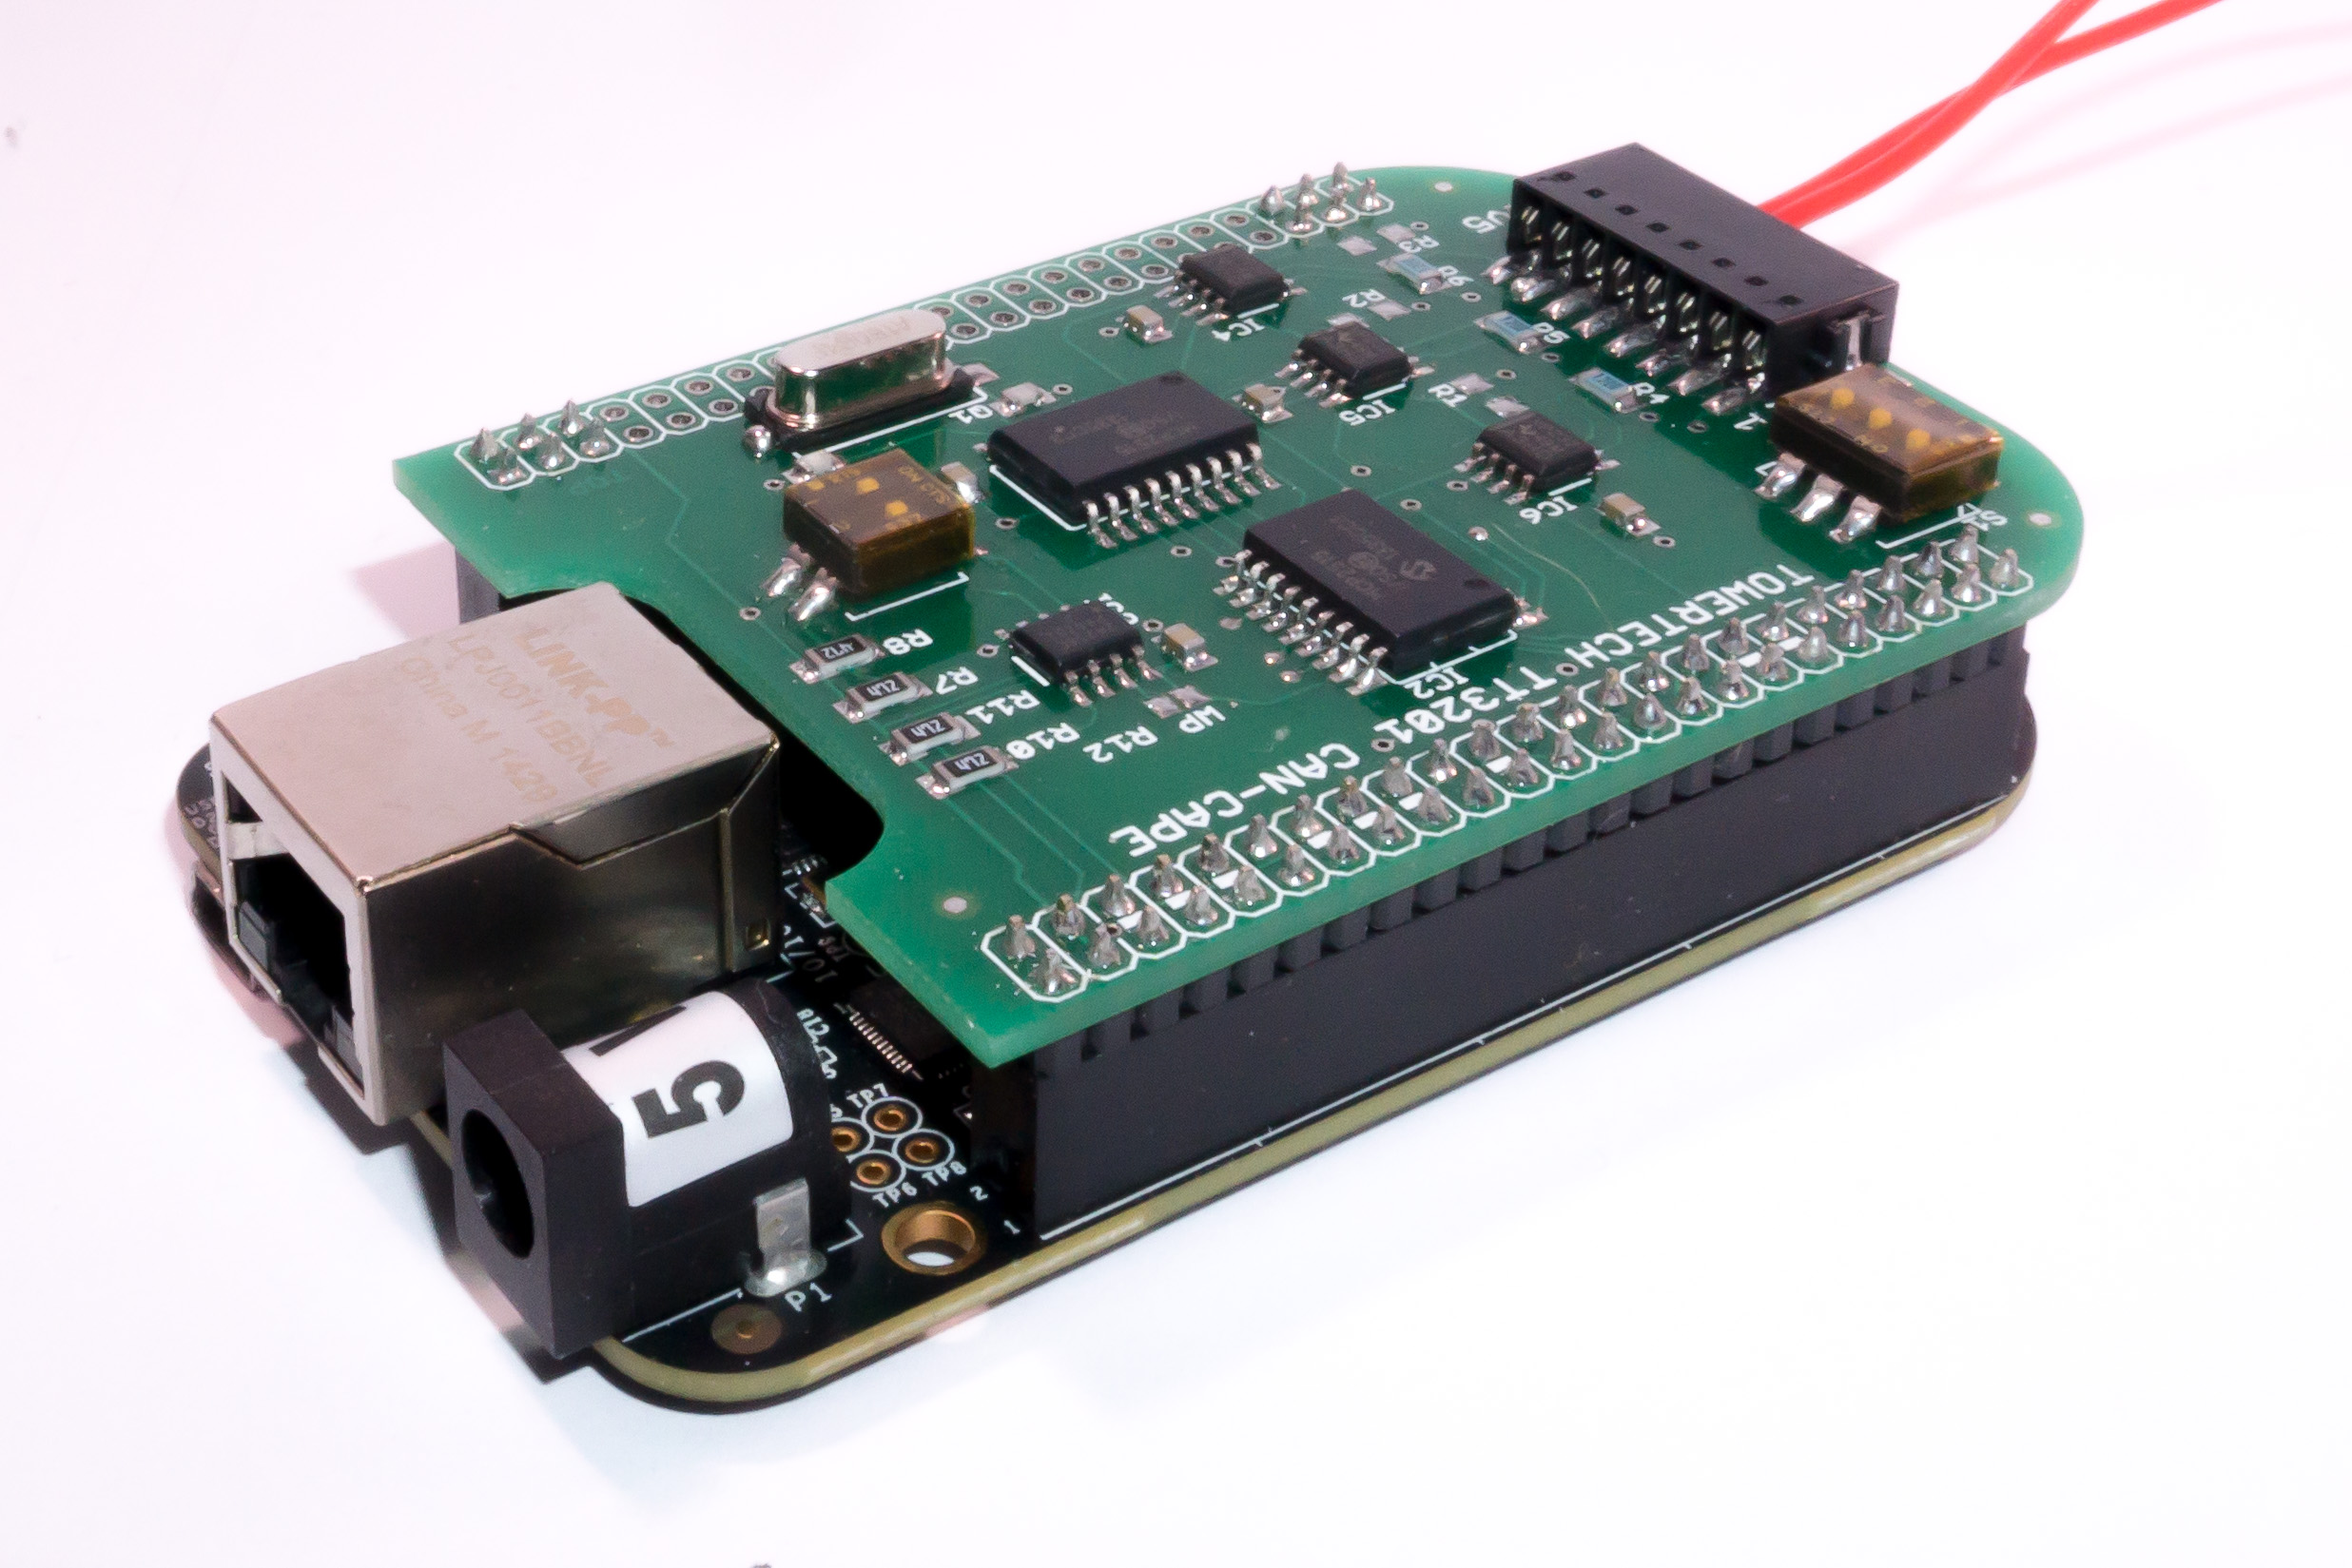
\includegraphics[width=\textwidth]{bilder/foto-4.jpg}
	\caption{Foto CanCape auf Bealge Bone Black}
	\label{fig:CanCape}
\end{figure}

%\textbf{Installationsinstruktionen siehe Anhang.}



\section{BLED112}
Die zweite Schnittstelle zu den Sensoren ist der USB Dongle BLED112 von Bluegiga. Dieser integriert den ganzen Bluetooth Smart Stack, der dank einer API über eine serielle Schnittstelle angesprochen werden kann.

\begin{figure}[hbtp]
	\center
	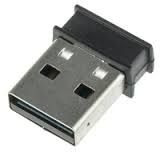
\includegraphics[width=4cm]{bilder/bled112.jpg}
	\caption{Foto BLED112}
	\label{fig:bled112}
\end{figure}

Die wichtigsten zu wissenden Details über den Bluegiga Dongle sind die folgenden:

\begin{itemize}
\itemsep 1pt \parskip 0pt \parsep 0pt
\item Kommunikation erfolgt über serielle Schnittstelle. Dem BLED112 werden darüber einfach die enstprechenden Anweisungen gesendet.

\item Material zu BLED112 (API Doku, Windows Treiber, Linux/Mac works out of the box) \url{https://www.bluegiga.com/en-US/products/bled112-bluetooth-smart-dongle/#documentation} → siehe im Speziellen API 1.3 Referenz


\item Java-LIB, wo die BLED 112 API bereits implementiert ist: \url{https://github.com/SINTEF-9012/bglib}


\item Ein paar Worte zum BLED112 selber:
	\begin{itemize}
	\itemsep 1pt \parskip 0pt \parsep 0pt
	\item  Das Teil ist programmierbarer Mikrocontroller mit komplett implementiertem Bluetooth-Stack, verpackt als USB-Dongle (Dongle = das D im BLED112)

	\item  Durch die Programmierung in Bluescript kann der Dongle unter anderem zu einem iBeacon gemacht werden.


	\item  Theoretisch bietet er aber viel mehr an. Er ist nebenbei ein direktes Konkurrenzprodukt zum nRF51 Chip von Nordic, der auf dem Sming zum Einsatz kommt.
	\end{itemize}


\item Beispiel-Befehlsabfolge, wie sie beim Sming zum Einsatz kommt. Detailbeschrieb der Parameter siehe Bluegiga API 1.3 Doku. Die Parameter-Werte entsprechen denen im Demo-Script und sollten lauffähig sein:

	\begin{itemize}
	\itemsep 1pt \parskip 0pt \parsep 0pt
	\item Suche nach BLE Advertisments
		\begin{itemize}
			\itemsep 1pt \parskip 0pt \parsep 0pt
			\item bg.api.gapSetScanParameters(0xC8, 0xC8, 0)
			\item bg.api.gapDiscover(1)
		\end{itemize}

	\item Wenn ein Device mit Name TXW51 gefunden, beende Suche kommt als Event mit Class = GenericAccessProfile siehe Demo-Script ab Zeile 238
		\begin{itemize}
			\itemsep 1pt \parskip 0pt \parsep 0pt
			\item Suche beenden: bg.api.gapEndProcedure()
		\end{itemize}
	

	\item Verbinde zum gefundenen Device anhand seiner MAC-Adresse
		\begin{itemize}
			\itemsep 1pt \parskip 0pt \parsep 0pt
			\item bg.api.gapConnectDirect( <MAC-Addr>, 1, 60, 76, 100, 9)
		\end{itemize}



	\item Hole einfach mal komplette Handle-Liste der Bluetooth Attribute (Optimieriungspotential da)
			\begin{itemize}
				\itemsep 1pt \parskip 0pt \parsep 0pt
				\item bg.api.attClientFindInformation( <connectionHandle>, 1, 0xffff)
			\end{itemize}


	\item Stimme die SMING UUIDs mit denen in der Handle-Liste überein. Merke zu jeder UUID deren Handle sowie UUID der CCID Attributes (siehe später)


	\item Lese mit den entsprechenden Handle das Attribut (ich habe einfach mal jeweils immmer gerade mal alle eingelesen)
			\begin{itemize}
				\itemsep 1pt \parskip 0pt \parsep 0pt
				\item bg.api.attClientReadByHandle(<connection>, <uuid handle> )
			\end{itemize}


	\item Zum Aktivieren der Accelometer-Messungen müssen folgende Attributte geschrieben werden:
			\begin{itemize}
				\itemsep 1pt \parskip 0pt \parsep 0pt
				\item bg.api.attClientAttributeWrite( <connection>, <uuid handle>, <newValue>)
				\item \url{LSM330_CHAR_GYRO_EN} = 1 
				\item \url{LSM330_CHAR_ACC_EN} = 1 
				\item \url{CCID UUID 0x02, 0x29 = 0x01, 0x00} ( Dies aktiviert das Bluetooth Feature CCID, wodruch das Sming bei Sming seitiger Attributwertänderung automatisch den neuen Wert sendet. Die Messwerte werden so per Push übertragen. Seitens Sming wird somit einfach der Messwert auf das Attribut \url{MEASURE_CHAR_DATASTREAM} geschrieben. Dies löst aus, dass der Bluetooth Stack des Smings automatisch den neue Messwert als Event zum Bluegiga Dongle übertragt und wir das so mitkriegen)
				\item \url{MEASURE_CHAR_START} = 1
			\end{itemize}


	\item Das Lesen der Temperatur muss mit einem Polling auf Attribut \url{LSM330_CHAR_TEMP_SAMPLE} gemacht werden.

	\item Beende Verbindung zum Sming
			\begin{itemize}
				\itemsep 1pt \parskip 0pt \parsep 0pt
				\item bg.api.connectionDisconnect( <connection> )
			\end{itemize}
	\end{itemize}
\end{itemize}
